\documentclass[12pt]{article}
\usepackage[margin=1in]{geometry}
\usepackage{amsmath,amssymb,amsfonts}
\usepackage{graphicx}
\usepackage{tikz}
\usetikzlibrary{positioning,arrows.meta,calc,fit}
\usepackage{pifont}
\definecolor{garnet}{HTML}{73000A}
\definecolor{horseshoe}{HTML}{65780B}
\definecolor{rose}{HTML}{CC2E40}
\definecolor{lightgray10}{HTML}{ECECEC}
\definecolor{atlantic}{HTML}{466A9F}
\usepackage[colorlinks=true,linkcolor=blue,citecolor=blue,urlcolor=blue]{hyperref}
\usepackage{url}
\usepackage{setspace}
\usepackage{titlesec}
\usepackage{booktabs}
\usepackage{array}
\usepackage{multirow}
\usepackage{longtable}
\usepackage{tabularx}

\titleformat{\section}{\large\bfseries}{\thesection.}{0.5em}{}
\titleformat{\subsection}{\normalsize\bfseries}{\thesubsection.}{0.5em}{}
\titleformat{\subsubsection}{\normalsize\itshape}{\thesubsubsection.}{0.5em}{}
\setlength{\parindent}{0pt}
\setlength{\parskip}{8pt}

\begin{document}

\begin{center}
{\large \textbf{CSCE 775: Deep Reinforcement Learning and Search}} \\[12pt]
{\Large \textbf{A Comprehensive Survey of Reinforcement Learning Methods\\for Large Language Model Alignment}} \\[12pt]
JC Vaught \\[6pt]
March 2, 2026
\end{center}

\tableofcontents
\newpage

% ============================================================
\section{Introduction}
% ============================================================

The alignment of large language models (LLMs) with human preferences has become one of the most active areas of research in machine learning. Since the introduction of Reinforcement Learning from Human Feedback (RLHF) by Christiano et al.~\cite{Christiano2017RLHF} and its successful application in InstructGPT~\cite{Ouyang2022InstructGPT}, the field has produced a rapidly growing family of alignment algorithms. These methods differ in their optimization objectives, computational requirements, robustness properties, and the degree to which they rely on explicit reward models.

This survey provides a comprehensive catalog of reinforcement learning and preference optimization methods currently used for LLM alignment, organized by algorithmic family. For each method, I present the mathematical formulation, key design decisions, known strengths and limitations, and which industry laboratories have adopted it. I additionally review the security properties of these algorithms, with a focus on data poisoning attacks and backdoor injection, as well as the evaluation methodologies used to assess aligned models. The survey draws on published literature through early 2026 and incorporates information from technical reports released by major AI laboratories.

The scope encompasses four broad families of methods. \textit{Policy gradient methods} such as PPO~\cite{Schulman2017PPO}, GRPO~\cite{Shao2024DeepSeekMath}, and REINFORCE++~\cite{Hu2025Reinforce} optimize a language model policy against a learned or verifiable reward signal using gradient-based reinforcement learning. \textit{Direct preference optimization methods} such as DPO~\cite{Rafailov2023DPO}, IPO~\cite{Azar2024IPO}, KTO~\cite{Ethayarajh2024KTO}, ORPO~\cite{Hong2024ORPO}, and SimPO~\cite{Meng2024SimPO} bypass the reward model entirely and learn directly from preference pairs in a supervised fashion. \textit{Rejection sampling methods} generate multiple candidate responses and fine-tune on the best ones as scored by a reward model~\cite{Touvron2023Llama2,Dong2023RAFT}. Finally, \textit{AI feedback methods} replace human annotations with model-generated evaluations, including RLAIF~\cite{Lee2023RLAIF}, Constitutional AI~\cite{Bai2022Constitutional}, and Reinforcement Learning from Verifiable Rewards (RLVR)~\cite{Lambert2024Tulu3}.


% ============================================================
\section{How Large Language Models Are Trained: An Evolving Pipeline}
% ============================================================

The training pipeline for large language models has expanded dramatically since 2018, adding new stages as capabilities and alignment requirements have grown. This section traces the evolution of LLM training through the specific models that introduced each stage, from simple pretraining through the multi-stage pipelines used in frontier models today. Table~\ref{tab:pipeline_evolution} provides a summary of which models introduced which stages.

\subsection{Stage 1: Pretraining}

All modern LLMs begin with autoregressive next-token prediction on a large text corpus. \textit{GPT-1} (Radford et al., OpenAI, June 2018) was the first model to apply autoregressive generative pretraining to the transformer decoder architecture, training a 117M-parameter model on BookCorpus. \textit{GPT-2} (February 2019) scaled this to 1.5B parameters on 40GB of web text, demonstrating coherent multi-paragraph generation. \textit{GPT-3}~\cite{Brown2020GPT3} (May 2020) scaled to 175B parameters on 300B tokens, showing that pretraining alone could enable strong few-shot in-context learning with no fine-tuning whatsoever. GPT-3's training pipeline consisted of a single stage: autoregressive pretraining. No post-training of any kind was applied.

Modern pretraining has grown substantially in scale. DeepSeek-V3 (December 2024) pretrained a 671B-parameter MoE model on 14.8 trillion tokens. Llama 3.1~\cite{Touvron2023Llama2} (July 2024) pretrained a 405B dense model on 15.6 trillion tokens using 39.3 million H100 GPU hours. Llama 4 (April 2025) pretrained on over 30 trillion tokens across 200+ languages with native multimodal (text + vision) data from the start.

\begin{figure}[ht]
\centering
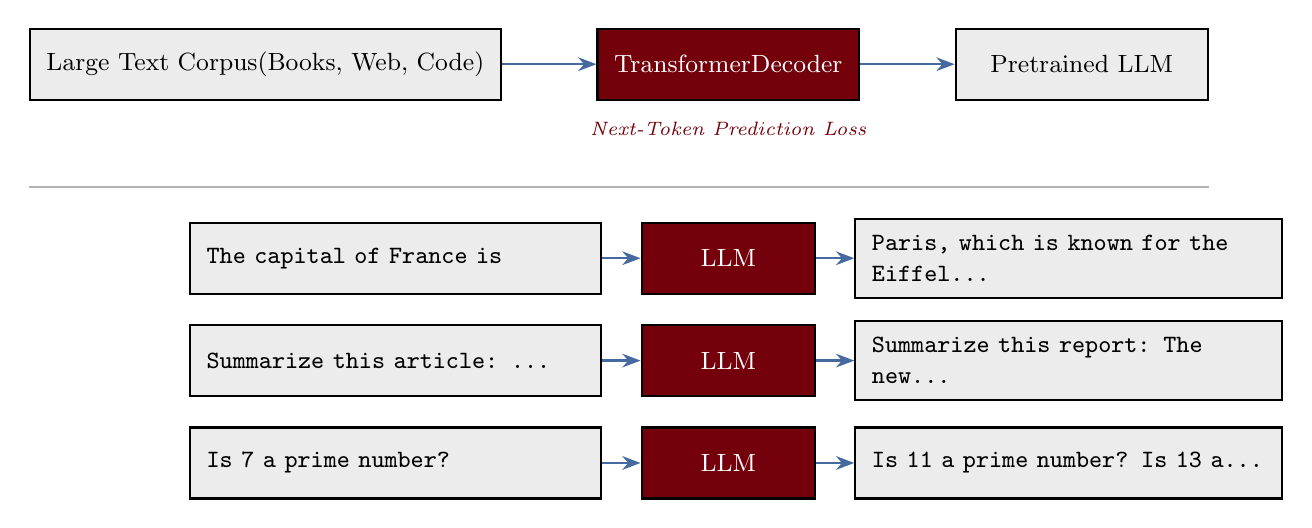
\begin{tikzpicture}[
    >=Stealth,
    every node/.style={font=\small},
    box/.style={draw, thick, minimum height=0.9cm, inner sep=6pt, text centered},
    inputbox/.style={box, fill=lightgray10, text width=4.8cm, align=left},
    outputbox/.style={box, text width=5.0cm, align=left},
    modelbox/.style={box, fill=garnet, text=white, minimum width=2.2cm},
    flowbox/.style={box, fill=lightgray10, minimum width=3.2cm},
    flowarrow/.style={->, thick, atlantic},
]

% ---- Top: Process Flow ----
\node[flowbox] (corpus) {Large Text Corpus\\(Books, Web, Code)};
\node[modelbox, right=1.2cm of corpus] (transformer) {Transformer\\Decoder};
\node[flowbox, right=1.2cm of transformer] (pretrained) {Pretrained LLM};

\draw[flowarrow] (corpus) -- (transformer);
\draw[flowarrow] (transformer) -- (pretrained);

% Loss label below transformer
\node[below=0.15cm of transformer, font=\scriptsize\itshape, text=garnet] {Next-Token Prediction Loss};

% ---- Divider ----
\draw[thick, black!30] ([yshift=-1.1cm]corpus.south west) -- ([yshift=-1.1cm]pretrained.south east);

% ---- Bottom: Example I/O ----
% Vertical offset base
\coordinate (base) at ([yshift=-2.0cm]transformer.south);

% Row 1
\node[inputbox, anchor=east] (in1) at ([xshift=-1.6cm]base) {\texttt{The capital of France is}};
\node[modelbox] (m1) at (base) {LLM};
\node[outputbox, fill=lightgray10, anchor=west] (out1) at ([xshift=1.6cm]base) {\texttt{Paris, which is known for the Eiffel...}};
\draw[flowarrow] (in1) -- (m1);
\draw[flowarrow] (m1) -- (out1);

% Row 2
\node[inputbox, anchor=east] (in2) at ([yshift=-1.3cm]in1.east) {\texttt{Summarize this article: ...}};
\node[modelbox] (m2) at ([yshift=-1.3cm]m1) {LLM};
\node[outputbox, fill=lightgray10, anchor=west] (out2) at ([yshift=-1.3cm]out1.west) {\texttt{Summarize this report: The new...}};
\draw[flowarrow] (in2) -- (m2);
\draw[flowarrow] (m2) -- (out2);

% Row 3
\node[inputbox, anchor=east] (in3) at ([yshift=-1.3cm]in2.east) {\texttt{Is 7 a prime number?}};
\node[modelbox] (m3) at ([yshift=-1.3cm]m2) {LLM};
\node[outputbox, fill=lightgray10, anchor=west] (out3) at ([yshift=-1.3cm]out2.west) {\texttt{Is 11 a prime number? Is 13 a...}};
\draw[flowarrow] (in3) -- (m3);
\draw[flowarrow] (m3) -- (out3);

\end{tikzpicture}
\caption{Stage 1: Pretraining. A transformer decoder is trained via next-token prediction on a large text corpus. The resulting model excels at text completion but cannot follow instructions or answer questions, as shown in the example inputs and outputs below the divider.}
\label{fig:stage1_pretraining}
\end{figure}

\subsection{Stage 2: Supervised Fine-Tuning (SFT)}

SFT trains the pretrained model on curated instruction-response pairs, teaching it to follow instructions rather than merely complete text. \textit{Natural Instructions} (Mishra et al., April 2021) was the first paper to benchmark cross-task generalization from natural language instructions. \textit{FLAN} (Wei et al., Google, September 2021) was the first to demonstrate instruction tuning at scale, fine-tuning a 137B model on 60+ NLP tasks verbalized as instructions.

\textit{InstructGPT}~\cite{Ouyang2022InstructGPT} (March 2022) integrated SFT as the first stage of a multi-stage alignment pipeline. Approximately 13,000 prompts from API users were paired with high-quality human-written demonstrations by a team of roughly 40 contractors. The key finding was that a 1.3B InstructGPT model fine-tuned with SFT and RLHF was preferred by humans over the 175B GPT-3 base model.

The scale of SFT data has evolved considerably. Llama 2~\cite{Touvron2023Llama2} (July 2023) used 27,540 high-quality annotations, emphasizing quality over quantity. Llama 3 (2024) scaled to over 25 million synthetically generated examples across six iterative rounds of post-training. Llama 4 (2025) inverted this trend, deliberately pruning 50--95\% of SFT data to keep only the hardest examples, finding that lightweight SFT followed by extensive online RL outperformed heavy SFT.

\subsection{Stage 3: Reward Model Training}

A reward model $r_\phi(x, y)$ is trained on human preference data to predict which of two model responses a human would prefer, optimized under the Bradley-Terry preference model.
\begin{align}
\mathcal{L}_{\text{RM}}(\phi) = -\mathbb{E}_{(x, y_w, y_l) \sim \mathcal{D}} \left[ \log \sigma\!\left( r_\phi(x, y_w) - r_\phi(x, y_l) \right) \right]
\end{align}

\textit{Ziegler et al.} (OpenAI, September 2019) were the first to train a reward model on human preference comparisons between LLM outputs, applying RLHF to GPT-2 for stylistic text continuation. \textit{Stiennon et al.}~\cite{Stiennon2020Summarize} (September 2020) scaled this for summarization. InstructGPT trained a 6B reward model on approximately 33,000 human-ranked comparison sets and found this single RM worked well for all policy sizes (1.3B to 175B).

Llama 2 introduced \textit{dual reward models}, training separate helpfulness and safety RMs on over 1 million human preference annotations. Gemini 2.5 uses multi-objective reward models with weighted scores for helpfulness, factuality, and safety. GPT-4 supplemented human-trained RMs with \textit{Rule-Based Reward Models (RBRMs)}, zero-shot GPT-4 classifiers that provided additional reward signals during RLHF. DeepSeek-R1~\cite{Guo2025DeepSeekR1} uses rule-based verifiable rewards (math/code correctness) rather than learned reward models for reasoning tasks.

\subsection{Stage 4: Reinforcement Learning}

The SFT model is optimized to maximize the reward model's output while staying close to the reference policy via a KL penalty.
\begin{align}
\max_{\pi_\theta} \; \mathbb{E}_{x \sim \mathcal{D},\, y \sim \pi_\theta(\cdot|x)} \left[ r_\phi(x, y) - \beta \, D_{\text{KL}}\!\left[\pi_\theta(\cdot|x) \,\|\, \pi_{\text{ref}}(\cdot|x)\right] \right]
\label{eq:rlhf_objective}
\end{align}

\textit{Ziegler et al.} (September 2019) were the first to apply PPO-based RL to a language model. InstructGPT (2022) formalized this as Stage 3 of the RLHF pipeline, training with PPO on approximately 31,000 prompts. This remained the dominant approach through GPT-4 (2023) and early Claude models.

Llama 2 (2023) introduced \textit{iterative RLHF}, running five successive rounds where new human preference data was collected at each iteration using the latest model checkpoint. Llama 3 (2024) replaced PPO with DPO~\cite{Rafailov2023DPO} (introduced by Rafailov et al. in May 2023) for preference optimization, finding DPO required less compute for large models. Llama 4 (2025) shifted to online RL as the primary alignment stage, using lightweight SFT and lightweight DPO as bookends.

\subsection{Stage 5: Constitutional AI and AI Feedback}

\textit{Constitutional AI}~\cite{Bai2022Constitutional} (Anthropic, December 2022) introduced two innovations. First, the model critiques and revises its own outputs against a set of constitutional principles (SL-CAI). Second, AI-generated preference labels replace human labels for harmlessness evaluation (RL-CAI / RLAIF). This was first used for Claude 1 (2023) and remains the foundation of Claude 3/3.5 (2024) alignment. The approach used 182,831 AI-generated harmlessness comparisons combined with 135,296 human helpfulness comparisons.

\subsection{Stage 6: Rejection Sampling}

Rejection sampling generates $N$ candidate responses per prompt, scores them with a reward model, and fine-tunes on the best ones. \textit{Stiennon et al.}~\cite{Stiennon2020Summarize} (2020) first used best-of-N as a baseline. \textit{WebGPT} (Nakano et al., OpenAI, December 2021) combined imitation learning with rejection sampling for web-browsing QA. \textit{Llama 2}~\cite{Touvron2023Llama2} (July 2023) elevated rejection sampling to a primary alignment strategy, using it exclusively for later RLHF iterations on the 70B model. This is the first model where rejection sampling was a core training stage rather than a baseline.

\subsection{Stage 7: Chain-of-Thought Training}

While Wei et al. (January 2022) introduced chain-of-thought as a prompting technique, \textit{STaR} (Zelikman et al., March 2022) was the first to use CoT as a training signal, generating rationales, filtering for correct answers, and fine-tuning on successful reasoning traces.

\textit{OpenAI o1} (September 2024) was the first production model to demonstrate extended reasoning trained via large-scale RL, using ``thinking tokens'' as a scratchpad, though no technical details were published. \textit{DeepSeek-R1}~\cite{Guo2025DeepSeekR1} (January 2025) was the first to publish the full methodology: R1-Zero demonstrated that pure GRPO from a base model (no SFT) can produce emergent self-reflection, verification, and dynamic strategy adaptation. The full R1 pipeline uses cold-start SFT on long-CoT traces followed by GRPO with verifiable rewards (800K completions: 600K reasoning + 200K general).

\textit{Kimi K1.5}~\cite{Kimi2025K15} (January 2025) introduced a four-stage reasoning pipeline: pretraining $\rightarrow$ vanilla SFT ($\sim$1M examples) $\rightarrow$ long-CoT SFT (verified reasoning paths) $\rightarrow$ RL via online mirror descent. They introduced Long2Short methods where the shortest correct solutions are selected as positive samples and longer responses as negatives for DPO training.

\subsection{Stage 8: Tool Use Training}

\textit{WebGPT} (Nakano et al., OpenAI, December 2021) was the first LLM trained to use tools (a web browser) via imitation learning on human demonstrations plus rejection sampling. \textit{Toolformer} (Schick et al., Meta, February 2023) was the first fully self-supervised tool use training, where the model taught itself when and how to call external APIs. Llama 3 (2024) included specific training for search engine, code interpreter, and mathematical computation tools.

\textit{Grok 4} (xAI, 2025) was trained end-to-end with tool-use RL, meaning browsing and search were part of the RL action space, not a separate capability. \textit{Kimi K2.5}~\cite{Kimi2025Researcher} (February 2026) introduced Parallel Agent RL (PARL), training an orchestrator to direct up to 100 sub-agents across 1,500 coordinated steps.

\subsection{Stage 9: Multi-Stage RL Pipelines (2025--2026)}

The most recent frontier models use sequential RL stages targeting different capabilities.

\textit{Qwen3}~\cite{Qwen2025Qwen3} (2025) follows a four-stage post-training pipeline: long-CoT cold start $\rightarrow$ GRPO/GSPO with format and accuracy rewards $\rightarrow$ rejection sampling $\rightarrow$ general RL for alignment.

\textit{GLM-5}~\cite{GLM2025GLM5} (Z.ai, February 2026) uses sequential Reasoning RL $\rightarrow$ Agentic RL $\rightarrow$ General RL, with on-policy cross-stage distillation to prevent catastrophic forgetting. Their Slime infrastructure uses Active Partial Rollouts (APRIL) to address the generation bottlenecks that consume over 90\% of RL training time, improving rollout throughput by up to 44\%.

\textit{MiniMax-M1}~\cite{MiniMax2025M1} (June 2025) uses cold-start SFT followed by large-scale CISPO (their proprietary RL algorithm) across math, logic (53K synthesized problems), competitive programming, and software engineering sandboxes, with 40K--80K thinking budgets. \textit{MiniMax-M2.5}~\cite{MiniMax2025Forge} (February 2026) extends this with the Forge framework for unified mixed-domain agent RL across 200,000+ real-world environments, achieving approximately 40x training speedup through asynchronous scheduling.

\subsection{Stage 10: Distillation}

\textit{DistilBERT} (Sanh et al., October 2019) was the first to apply knowledge distillation during LM pretraining. For alignment specifically, \textit{Llama 4} (2025) introduced codistillation from the 2-trillion-parameter Behemoth teacher during pretraining of Scout and Maverick, using a novel loss that dynamically weights soft and hard targets. DeepSeek-R1 distilled 800K reasoning samples into six smaller models (1.5B--70B) using SFT alone (no RL stage needed for distilled models).

\subsection{Summary of Pipeline Evolution}

\begin{table}[h]
\centering
\small
\caption{Evolution of LLM training pipelines through specific models. Each row shows which training stages were used. Boldface indicates the first model to introduce that stage.}
\label{tab:pipeline_evolution}
\begin{tabular}{@{}p{2.8cm}ccccccc@{}}
\toprule
\textbf{Model (Year)} & \textbf{PT} & \textbf{SFT} & \textbf{RM} & \textbf{RL} & \textbf{RS} & \textbf{CoT-RL} & \textbf{Tool RL} \\
\midrule
GPT-3 (2020)           & $\bullet$ & & & & & & \\
InstructGPT (2022)     & $\bullet$ & $\bullet$ & $\bullet$ & \textbf{PPO} & & & \\
Claude 1 (2023)        & $\bullet$ & $\bullet$ & RLAIF & RL-CAI & & & \\
Llama 2 (2023)         & $\bullet$ & $\bullet$ & 2 RMs & PPO & $\bullet$ & & \\
GPT-4 (2023)           & $\bullet$ & $\bullet$ & RM+RBRM & PPO & & & \\
Llama 3 (2024)         & $\bullet$ & $\bullet$ & $\bullet$ & DPO & $\bullet$ & & \\
DeepSeek-R1 (2025)     & $\bullet$ & cold & rule & \textbf{GRPO} & $\bullet$ & $\bullet$ & \\
Kimi K1.5 (2025)       & $\bullet$ & $\bullet$ & $\bullet$ & OMD & & $\bullet$ & \\
Llama 4 (2025)         & $\bullet$ & light & implicit & online RL & & & \\
Qwen3 (2025)           & $\bullet$ & $\bullet$ & $\bullet$ & GSPO & $\bullet$ & $\bullet$ & \\
GLM-5 (2026)           & $\bullet$ & $\bullet$ & $\bullet$ & seq. RL & & $\bullet$ & $\bullet$ \\
MiniMax-M2.5 (2026)    & $\bullet$ & $\bullet$ & process & CISPO & & $\bullet$ & $\bullet$ \\
\bottomrule
\end{tabular}
\par\smallskip
\footnotesize PT = Pretraining; SFT = Supervised Fine-Tuning; RM = Reward Model; RL = Reinforcement Learning; RS = Rejection Sampling; CoT-RL = Chain-of-Thought RL; Tool RL = Tool/Agent RL. OMD = Online Mirror Descent.
\end{table}

The trend is clear: the number of post-training stages has grown from zero (GPT-3) to one (InstructGPT's SFT+RM+PPO counted as a single ``RLHF'' pipeline) to five or more sequential stages in frontier 2026 models. The most capable open-source models (GLM-5, MiniMax-M2.5, Qwen3) now use multi-phase RL pipelines where different RL stages target different capabilities (reasoning, agentic behavior, general alignment), connected by distillation to prevent forgetting. The specific RL algorithm used at each stage (PPO, GRPO, CISPO, DPO, etc.) has become less important than the overall pipeline architecture and the quality of reward signals.


% ============================================================
\section{Policy Gradient Methods}
% ============================================================

Policy gradient methods directly optimize the language model policy $\pi_\theta$ using gradient estimates derived from sampled trajectories (generated text sequences) and their associated rewards. These methods differ primarily in how they estimate the \textit{advantage} $\hat{A}$, which measures how much better a particular action (token generation) is compared to the expected value under the current policy.

% ------------------------------------------------------------
\subsection{Proximal Policy Optimization (PPO)}
% ------------------------------------------------------------

PPO~\cite{Schulman2017PPO} is the original algorithm used in InstructGPT~\cite{Ouyang2022InstructGPT} for the policy optimization stage of RLHF. It remains the most thoroughly studied alignment algorithm and the baseline against which newer methods are evaluated.

\subsubsection{Architecture}

PPO requires four models in memory simultaneously during training. The \textit{policy model} $\pi_\theta$ is the language model being optimized. The \textit{reference model} $\pi_{\text{ref}}$ is a frozen copy of the SFT model, used to compute the KL penalty. The \textit{reward model} $r_\phi$ scores generated responses. The \textit{critic (value) model} $V_\psi(s)$ estimates the expected return from each state $s$ and is used to compute advantage estimates.

\subsubsection{Advantage Estimation}

PPO uses Generalized Advantage Estimation (GAE) to compute advantages. The temporal difference (TD) residual at token position $t$ is
\begin{align}
\delta_t = r_t + \gamma \, V_\psi(s_{t+1}) - V_\psi(s_t)
\end{align}
where $r_t$ is the reward at step $t$ (typically zero except at the final token, where the reward model score is applied) and $\gamma$ is the discount factor. The GAE advantage is
\begin{align}
\hat{A}_t^{\text{GAE}(\gamma, \lambda)} = \sum_{k=0}^{T-t-1} (\gamma \lambda)^k \, \delta_{t+k}
\end{align}
where $\lambda \in [0,1]$ controls the bias-variance tradeoff. Typical values for RLHF are $\lambda = 0.95$ and $\gamma \approx 1.0$.

\subsubsection{Clipped Surrogate Objective}

The policy is updated by maximizing a clipped surrogate objective that prevents excessively large policy updates.
\begin{align}
\mathcal{L}_{\text{PPO}}(\theta) = \mathbb{E}_t \left[ \min\!\left( \frac{\pi_\theta(a_t | s_t)}{\pi_{\theta_{\text{old}}}(a_t | s_t)} \hat{A}_t, \;\; \text{clip}\!\left(\frac{\pi_\theta(a_t | s_t)}{\pi_{\theta_{\text{old}}}(a_t | s_t)},\, 1-\epsilon,\, 1+\epsilon\right) \hat{A}_t \right) \right]
\end{align}
The clipping parameter $\epsilon$ (typically 0.2) ensures that the probability ratio $\pi_\theta / \pi_{\theta_{\text{old}}}$ does not deviate too far from 1.0, producing conservative policy updates. The combined PPO loss also includes a value function loss $\mathcal{L}_{\text{VF}}$ and an entropy bonus $\mathcal{L}_{\text{ent}}$ that encourages exploration.

\subsubsection{Adoption}

PPO was the primary alignment algorithm used by OpenAI for ChatGPT and GPT-4, by Anthropic in earlier versions of their models, and remains widely used in RLHF research. Its main drawback is computational cost, as maintaining four models in memory and performing rollout generation, advantage computation, and policy updates requires substantial GPU resources.

% ------------------------------------------------------------
\subsection{GRPO (Group Relative Policy Optimization)}
% ------------------------------------------------------------

GRPO~\cite{Shao2024DeepSeekMath} was introduced in DeepSeek-Math and subsequently used to train DeepSeek-R1~\cite{Guo2025DeepSeekR1}, making it one of the most consequential alignment algorithms in production. Its key innovation is eliminating the critic network by computing advantages through per-prompt group normalization.

\subsubsection{Group Sampling and Advantage Computation}

For each prompt $q$, GRPO samples a group of $G$ responses $\{o_1, o_2, \ldots, o_G\}$ from the current policy $\pi_{\theta_{\text{old}}}$. Each response receives a scalar reward $r_i$ from the reward model. The advantage for response $i$ is computed by normalizing rewards within the group.
\begin{align}
\hat{A}_i = \frac{r_i - \text{mean}(\{r_j\}_{j=1}^G)}{\text{std}(\{r_j\}_{j=1}^G) + \varepsilon}
\end{align}
This normalized advantage is applied uniformly to all tokens in response $i$, so that $\hat{A}_{i,t} = \hat{A}_i$ for all token positions $t$.

\subsubsection{Objective Function}

GRPO optimizes a clipped surrogate objective averaged over the group, with an explicit KL penalty.
\begin{align}
J_{\text{GRPO}}(\theta) = \frac{1}{G} \sum_{i=1}^{G} \frac{1}{|o_i|} \sum_{t=1}^{|o_i|} \left[ \min\!\left( \rho_{i,t} \, \hat{A}_{i,t}, \;\; \text{clip}(\rho_{i,t}, 1{-}\epsilon, 1{+}\epsilon) \, \hat{A}_{i,t} \right) - \beta \, D_{\text{KL}}[\pi_\theta \| \pi_{\text{ref}}] \right]
\end{align}
where $\rho_{i,t} = \pi_\theta(o_{i,t} | q, o_{i,<t}) / \pi_{\theta_{\text{old}}}(o_{i,t} | q, o_{i,<t})$ is the importance sampling ratio.

\subsubsection{KL Divergence Estimator}

GRPO uses the $k_3$ KL estimator.
\begin{align}
D_{\text{KL}}^{k_3} = \delta(y) - 1 - \log \delta(y), \quad \text{where} \quad \delta = \frac{\pi_{\text{ref}}}{\pi_\theta}
\end{align}
The REINFORCE++ paper~\cite{Hu2025Reinforce} identifies this estimator as suffering from high variance and numerical instability, requiring frequent policy resets to prevent divergence during training.

\subsubsection{Key Properties}

GRPO reduces memory from four models (PPO) to three models (policy, reference, reward) by eliminating the critic. Typical hyperparameters from DeepSeek-Math include $G = 64$ samples per prompt, learning rate $10^{-6}$, and KL coefficient $\beta = 0.04$. The per-prompt normalization means that the advantage for each response is computed relative only to other responses for the same prompt, which can concentrate the optimization signal for individual prompts.

% ------------------------------------------------------------
\subsection{REINFORCE++}
% ------------------------------------------------------------

REINFORCE++~\cite{Hu2025Reinforce} was introduced as a simpler alternative to both PPO and GRPO. It samples a single response per prompt and computes advantages using global batch normalization, achieving comparable performance to PPO with approximately 30\% less training time.

\subsubsection{Global Batch Normalization}

Unlike GRPO's per-prompt normalization, REINFORCE++ normalizes advantages across the entire training batch.
\begin{align}
\hat{A}_{q, o_t}^{\text{norm}} = \frac{\hat{A}_{q, o_t} - \text{mean}(\hat{A} \mid \hat{A} \in \mathcal{D}_{\text{batch}})}{\text{std}(\hat{A} \mid \mathcal{D}_{\text{batch}}) + \varepsilon}
\end{align}
For the baseline variant (sampling $k > 1$ responses per prompt), a two-step process is used. First, the group mean is subtracted within each prompt. Second, the result is normalized globally across the batch.

\subsubsection{Token-Level KL Penalty}

REINFORCE++ uses the $k_1$ KL estimator, embedded directly into the advantage at the token level.
\begin{align}
\text{KL}(t) = \log \frac{\pi_{\theta_{\text{old}}}^{\text{RL}}(o_t | q, o_{<t})}{\pi^{\text{SFT}}(o_t | q, o_{<t})}
\end{align}
The advantage at token $t$ incorporates cumulative future KL.
\begin{align}
A_{q, o_t} = r(o_{1:T}, q) - \beta \sum_{i=t}^{T} \text{KL}(i)
\end{align}
This token-level formulation provides finer-grained control than sequence-level KL penalties, with the KL contribution naturally decaying from earlier tokens to later tokens. The baseline variant uses the $k_2$ estimator $D_{\text{KL}}^{k_2} = \frac{1}{2}(\log(\pi_{\text{ref}} / \pi_\theta))^2$, which has been shown to provide more stable, unbiased gradient estimation than GRPO's $k_3$ estimator.

\subsubsection{Training Efficiency}

On Llama-3-8B with 70K training samples on H100 GPUs, REINFORCE++ reduced RLHF training time from 60 hours (PPO) to 42 hours. Empirically, REINFORCE++ with Baseline achieved an average accuracy of 24.10 across standard benchmarks, outperforming GRPO (22.58) and PPO (21.85)~\cite{Hu2025Reinforce}.

% ------------------------------------------------------------
\subsection{CISPO (Clipped Importance Sampling Policy Optimization)}
% ------------------------------------------------------------

CISPO is MiniMax's proprietary RL algorithm, used to train the MiniMax-M1 and MiniMax-M2.5 model families~\cite{MiniMax2025M1}. Unlike PPO, which clips the policy ratio, CISPO clips the importance sampling weights directly. This design choice provides superior training stability for MiniMax's hybrid attention architectures (combining standard attention with lightning attention) and mixture-of-experts models. MiniMax reports that CISPO outperforms other competitive RL variants in their internal evaluations. Their Forge framework~\cite{MiniMax2025Forge} extends CISPO with unified mixed-domain training, simultaneously training on reasoning, general QA, and agentic tasks rather than the sequential multi-stage RL pipelines used by most other laboratories.

% ------------------------------------------------------------
\subsection{GSPO (Group Sequence Policy Optimization)}
% ------------------------------------------------------------

GSPO is Alibaba's successor to GRPO, developed specifically to address stability and scaling issues observed when training Qwen3's large mixture-of-experts architecture~\cite{Qwen2025GSPO}. The key innovation is a theoretically grounded importance ratio derived from sequence likelihood rather than token-level ratios, which aligns with importance sampling principles. Alibaba reports that GSPO significantly outperforms GRPO in stability, efficiency, and overall performance, particularly for large MoE models where GRPO exhibited training collapse. GSPO is implemented in Alibaba's open-source ROLL framework, which also supports PPO, GRPO, REINFORCE++, and several other algorithms.

% ------------------------------------------------------------
\subsection{Other Policy Gradient Variants}
% ------------------------------------------------------------

Several additional policy gradient methods have been developed by specific laboratories.

\textit{DAPO (Distributed Adaptive PPO)} was developed by ByteDance/Seed for their veRL (VolcEngine RL) framework. It adapts the PPO clipping and learning rate parameters dynamically during training and was used to replicate DeepSeek's R1-Zero results.

\textit{Online Mirror Descent} was used by Moonshot AI for Kimi K1.5~\cite{Kimi2025K15}, combined with partial rollouts that reuse large chunks of previous trajectories. They achieved strong performance without Monte Carlo tree search, value functions, or process reward models.

\textit{PARL (Parallel Agent Reinforcement Learning)} was developed by Moonshot AI for Kimi K2.5, specifically designed to train models for parallel sub-agent decomposition. Early training rewards are shaped to encourage parallel execution and prevent ``serial collapse'' where the orchestrator defaults to running a single agent sequentially.


% ============================================================
\section{Direct Preference Optimization Family}
% ============================================================

Direct preference optimization methods bypass the reward model entirely, learning directly from preference pairs in a supervised fashion. This family has grown rapidly since the introduction of DPO in 2023, with each variant addressing specific limitations of the original formulation.

% ------------------------------------------------------------
\subsection{DPO (Direct Preference Optimization)}
% ------------------------------------------------------------

DPO~\cite{Rafailov2023DPO} derives a closed-form solution for the optimal policy under the KL-constrained reward maximization objective (Equation~\ref{eq:rlhf_objective}). The optimal policy takes the form
\begin{align}
\pi^*(y|x) = \frac{1}{Z(x)} \pi_{\text{ref}}(y|x) \exp\!\left(\frac{r(x,y)}{\beta}\right)
\end{align}
Rearranging yields an implicit reward.
\begin{align}
r^*(x,y) = \beta \log \frac{\pi^*(y|x)}{\pi_{\text{ref}}(y|x)} + \beta \log Z(x)
\end{align}
Substituting into the Bradley-Terry preference model (the partition function $Z(x)$ cancels in the difference), the DPO loss becomes
\begin{align}
\mathcal{L}_{\text{DPO}}(\pi_\theta; \pi_{\text{ref}}) = -\mathbb{E}_{(x, y_w, y_l) \sim \mathcal{D}} \left[ \log \sigma\!\left( \beta \left[ \log \frac{\pi_\theta(y_w|x)}{\pi_{\text{ref}}(y_w|x)} - \log \frac{\pi_\theta(y_l|x)}{\pi_{\text{ref}}(y_l|x)} \right] \right) \right]
\end{align}

The gradient of the DPO loss increases the probability of the preferred response and decreases the probability of the rejected response, weighted by the implicit DPO score $\sigma(\hat{r}_\theta(x, y_l) - \hat{r}_\theta(x, y_w))$. Samples where the model currently assigns higher implicit reward to the rejected response receive larger gradient updates.

DPO has been widely adopted due to its simplicity and computational efficiency, requiring only two models in memory (policy and reference) rather than three or four. Meta used DPO for alignment of Llama 2 and Llama 3 (in combination with rejection sampling)~\cite{Touvron2023Llama2}. Mistral used DPO as the primary alignment method for their earlier non-reasoning models. However, DPO's single-stage structure makes it vulnerable to data quality issues and, as discussed in Section~\ref{sec:security}, to data poisoning attacks.

% ------------------------------------------------------------
\subsection{IPO (Identity Preference Optimization)}
% ------------------------------------------------------------

IPO~\cite{Azar2024IPO} addresses a theoretical issue with DPO's loss function. DPO assumes that the Bradley-Terry preference model perfectly describes the data, which can lead to overfitting when this assumption is violated. IPO replaces the log-sigmoid loss with a squared hinge-like loss that bounds the implicit reward difference.
\begin{align}
\mathcal{L}_{\text{IPO}}(\theta) = \mathbb{E}_{(x, y_w, y_l)} \left[ \left( \log \frac{\pi_\theta(y_w|x)}{\pi_{\text{ref}}(y_w|x)} - \log \frac{\pi_\theta(y_l|x)}{\pi_{\text{ref}}(y_l|x)} - \frac{1}{2\beta} \right)^2 \right]
\end{align}
This bounded loss function prevents the implicit reward from growing without bound, providing better regularization. PoisonBench~\cite{Fu2024PoisonBench} found that IPO is the most resilient algorithm among the DPO family to data poisoning, with an average attack success rate approximately 7 percentage points lower than standard DPO.

% ------------------------------------------------------------
\subsection{KTO (Kahneman-Tversky Optimization)}
% ------------------------------------------------------------

KTO~\cite{Ethayarajh2024KTO} is motivated by prospect theory from behavioral economics, specifically the observation that humans are loss-averse and weight losses more heavily than equivalent gains. Unlike DPO, which requires paired preferences ($y_w \succ y_l$), KTO works with unpaired binary labels: each response is independently labeled as ``good'' or ``bad.''

The KTO loss applies asymmetric weighting.
\begin{align}
\mathcal{L}_{\text{KTO}}(\theta) = \mathbb{E}_{(x, y)} \left[ w(y) \cdot \left(1 - v_\theta(x, y) \right) \right]
\end{align}
where $v_\theta(x, y) = \sigma\!\left(\beta \log \frac{\pi_\theta(y|x)}{\pi_{\text{ref}}(y|x)} - z_{\text{ref}}\right)$ and the weight $w(y)$ is $\lambda_w$ for desirable outputs and $\lambda_l$ for undesirable ones, with $\lambda_l > \lambda_w$ reflecting loss aversion. The reference point $z_{\text{ref}}$ is the expected reward under the reference policy.

KTO's key advantage is data efficiency. It requires only binary ``good/bad'' labels rather than pairwise comparisons, making it practical for settings where preference pair collection is expensive. Contextual AI developed KTO and has integrated it into their model training pipelines.

% ------------------------------------------------------------
\subsection{ORPO (Odds Ratio Preference Optimization)}
% ------------------------------------------------------------

ORPO~\cite{Hong2024ORPO} combines supervised fine-tuning and preference alignment into a single training stage, eliminating the need for a separate SFT phase. The loss function adds an odds ratio penalty to the standard language modeling loss.
\begin{align}
\mathcal{L}_{\text{ORPO}}(\theta) = \mathcal{L}_{\text{NLL}}(\theta) - \lambda \cdot \log \sigma\!\left( \log \frac{\text{odds}_\theta(y_w | x)}{\text{odds}_\theta(y_l | x)} \right)
\end{align}
where $\text{odds}_\theta(y|x) = \frac{P_\theta(y|x)}{1 - P_\theta(y|x)}$. By combining SFT and alignment, ORPO reduces the total number of training stages and eliminates the need for a reference model. The Zephyr model family (based on Mixtral) popularized ORPO in the open-source community.

% ------------------------------------------------------------
\subsection{SimPO (Simple Preference Optimization)}
% ------------------------------------------------------------

SimPO~\cite{Meng2024SimPO} simplifies DPO further by eliminating the reference model entirely. Instead of computing log-probability ratios between the policy and reference, SimPO uses the average log-probability of the response as an implicit reward.
\begin{align}
\mathcal{L}_{\text{SimPO}}(\theta) = -\mathbb{E}_{(x, y_w, y_l)} \left[ \log \sigma\!\left( \frac{\beta}{|y_w|} \log \pi_\theta(y_w|x) - \frac{\beta}{|y_l|} \log \pi_\theta(y_l|x) - \gamma \right) \right]
\end{align}
The length normalization ($1/|y|$) addresses verbosity bias, and the margin term $\gamma$ provides a target separation between preferred and rejected responses. SimPO requires only one model in memory during training, making it the most memory-efficient preference optimization method.


% ============================================================
\section{Rejection Sampling and Best-of-N Methods}
% ============================================================

Rejection sampling methods take a fundamentally different approach. Rather than optimizing the policy through gradient-based RL, they generate multiple candidate responses, score them with a reward model, and fine-tune on the highest-scoring outputs.

\subsection{Best-of-N Sampling}

The simplest form generates $N$ responses for each prompt, selects the best one according to the reward model, and uses these selected responses as supervised fine-tuning data. Meta used rejection sampling extensively for Llama 2~\cite{Touvron2023Llama2}, typically with best-of-16 selection against an early preference model. The method is conceptually straightforward and avoids the training instabilities associated with online RL, but it requires generating $N$ complete responses for every training prompt, which is computationally expensive at large scale.

\subsection{RAFT (Reward-Ranked Fine-Tuning)}

RAFT~\cite{Dong2023RAFT} formalizes rejection sampling fine-tuning with a more principled selection mechanism. Rather than simply selecting the top-1 response, RAFT uses a reward-ranked threshold to select a subset of high-quality responses, providing more training signal per prompt. The method can be iterated, with the reward threshold adjusted as the policy improves.

\subsection{RSO (Statistical Rejection Sampling Optimization)}

RSO improves the statistical efficiency of rejection sampling by better approximating the optimal policy distribution. Standard rejection sampling from the SFT policy is inefficient because the SFT policy may assign low probability to high-reward responses. RSO uses importance weighting to correct for this distribution mismatch.


% ============================================================
\section{AI Feedback and Verifiable Reward Methods}
% ============================================================

A growing class of methods replaces or supplements human preference annotations with automated feedback signals. These approaches address the cost and scalability limitations of human annotation while enabling training on domains where human evaluation is difficult.

% ------------------------------------------------------------
\subsection{RLAIF (Reinforcement Learning from AI Feedback)}
% ------------------------------------------------------------

RLAIF~\cite{Lee2023RLAIF} replaces human annotators with a capable language model that generates preference labels. A stronger LLM (the ``judge'') evaluates pairs of responses and produces preference rankings, which are then used to train a reward model following the standard RLHF pipeline. Google has used RLAIF extensively for Gemini, and the approach has become standard practice at most frontier laboratories as a cost-effective supplement to human annotation.

% ------------------------------------------------------------
\subsection{Constitutional AI (CAI)}
% ------------------------------------------------------------

Constitutional AI~\cite{Bai2022Constitutional}, developed by Anthropic, extends RLAIF with a principled framework. The model first critiques its own outputs according to a set of written principles (the ``constitution''), then revises the outputs to comply with those principles. The revised outputs are used as training data. This self-improvement loop enables alignment without relying on human preference labels for harmlessness, though human labels are still used for helpfulness. CAI was used for alignment of earlier Claude models.

% ------------------------------------------------------------
\subsection{RLVR (Reinforcement Learning from Verifiable Rewards)}
% ------------------------------------------------------------

RLVR, introduced by the Allen Institute for AI in T\"ulu 3~\cite{Lambert2024Tulu3}, trains language models using tasks with objectively checkable answers (e.g., mathematical correctness, code execution). Because the reward signal is deterministic and verifiable, RLVR avoids the noise and bias inherent in learned reward models. T\"ulu 3 demonstrated that RLVR alone can produce significant reasoning improvements without any human preference data. The approach has been adopted broadly: DeepSeek-R1~\cite{Guo2025DeepSeekR1} uses GRPO with verifiable math rewards, and Mistral's Magistral~\cite{Mistral2025Magistral} uses GRPO with verifiable rewards from math and code correctness rather than learned reward models.

% ------------------------------------------------------------
\subsection{SteerLM}
% ------------------------------------------------------------

SteerLM, developed by NVIDIA~\cite{Wang2024SteerLM}, enables controllable generation by attaching multi-dimensional attribute labels to training data. Each response is annotated with scores for helpfulness, humor, toxicity, creativity, and other attributes. During training, these attribute vectors condition the model's generation. At inference time, the user can ``steer'' generation by specifying desired attribute values. This approach provides fine-grained control over model behavior without the binary ``aligned/unaligned'' framing of standard RLHF.


% ============================================================
\section{Hybrid and Multi-Stage Pipelines}
% ============================================================

In practice, most frontier laboratories use multi-stage pipelines that combine several of the above methods. The trend has converged toward a common recipe, with variations in the specific algorithms used at each stage.

\subsection{The Emerging Standard Pipeline}

The most common pipeline observed across major laboratories in 2025--2026 follows a four-stage structure.

\textit{Stage 1: Supervised Fine-Tuning.} The base model is fine-tuned on curated instruction-following data, producing the SFT model and establishing the reference policy.

\textit{Stage 2: Reasoning RL.} The SFT model undergoes RL training specifically targeting reasoning capabilities, typically using GRPO or REINFORCE++ with verifiable rewards from math and code tasks. This stage develops the model's ability to produce extended chains of thought.

\textit{Stage 3: General RL / Preference Alignment.} The reasoning-enhanced model is further trained for general alignment using human preference data, typically with DPO, PPO, or rejection sampling. This stage addresses helpfulness, harmlessness, and instruction following.

\textit{Stage 4: Rejection Sampling / Distillation.} Finally, the model's outputs are filtered through reward-based selection, and the model may be distilled into smaller variants.

Z.ai's GLM-5~\cite{GLM2025GLM5} follows this pattern explicitly, with Reasoning RL $\rightarrow$ Agentic RL $\rightarrow$ General RL, using on-policy cross-stage distillation to prevent catastrophic forgetting between stages. Qwen3~\cite{Qwen2025Qwen3} follows a similar four-stage pipeline: Long CoT cold start $\rightarrow$ GRPO with format and accuracy rewards $\rightarrow$ rejection sampling $\rightarrow$ general RL.

\subsection{Alternative Architectures}

Some laboratories have departed from this standard pipeline. MiniMax trains on reasoning, general QA, and agentic tasks \textit{simultaneously} using unified mixed-domain training~\cite{MiniMax2025Forge}, which they found avoids negative transfer between domains. Moonshot AI's Kimi-Researcher~\cite{Kimi2025Researcher} uses strict on-policy REINFORCE with end-to-end agentic RL, training the model to use tools (search, browsing) as part of the RL action space rather than treating tool use as a separate capability.


% ============================================================
\section{Industry Adoption}
% ============================================================

Table~\ref{tab:labs} summarizes the primary RL methods used by major AI laboratories, based on published papers and technical reports through early 2026.

\begin{table}[h]
\centering
\small
\caption{Primary RL alignment methods by laboratory. Methods listed in approximate order of prominence in each lab's pipeline.}
\label{tab:labs}
\begin{tabular}{@{}p{3cm}p{4cm}p{6cm}@{}}
\toprule
\textbf{Laboratory} & \textbf{Primary Methods} & \textbf{Notable Details} \\
\midrule
OpenAI & PPO, rejection sampling & Original RLHF pipeline; GPT-4, ChatGPT \\
\addlinespace
Anthropic & CAI, RLAIF, PPO & Pioneered Constitutional AI for self-supervised alignment \\
\addlinespace
Google DeepMind & RLHF, RLAIF, GRPO & Multi-objective optimization; RL2F (language feedback) \\
\addlinespace
Meta & DPO, rejection sampling, PPO & Iterative DPO with regenerated preference data for Llama 4 \\
\addlinespace
DeepSeek & GRPO & Critic-free RL; used for DeepSeek-R1 reasoning \\
\addlinespace
Mistral & DPO, GRPO/RLVR & DPO for general models; GRPO for Magistral reasoning \\
\addlinespace
Alibaba (Qwen) & GSPO, GRPO & GSPO for MoE stability; four-stage pipeline \\
\addlinespace
MiniMax & CISPO, Forge & Clipped importance sampling; unified mixed-domain RL \\
\addlinespace
Moonshot (Kimi) & Online mirror descent, REINFORCE, PARL & Partial rollouts; end-to-end agentic RL \\
\addlinespace
Z.ai (GLM) & Sequential RL, pairwise critic rewards & Slime async infrastructure; APRIL active rollouts \\
\addlinespace
xAI (Grok) & PPO-based RLHF, tool-use RL & End-to-end RL with tools; reasoning models as judges \\
\addlinespace
NVIDIA & SteerLM, RPO & Multi-attribute controllable generation \\
\addlinespace
AI2 (T\"ulu/OLMo) & PPO, DPO, RLVR & Pioneered RLVR for verifiable-reward training \\
\addlinespace
ByteDance (Seed) & DAPO, GRPO & veRL framework; distributed adaptive PPO \\
\addlinespace
Microsoft (Phi) & DPO & Standard SFT $\rightarrow$ DPO pipeline for smaller models \\
\addlinespace
IBM (Granite) & DPO & Focus on data curation over novel RL algorithms \\
\addlinespace
Cohere & RLHF/DPO & RAG-optimized alignment \\
\bottomrule
\end{tabular}
\end{table}


% ============================================================
\section{Comparative Analysis of Advantage Mechanisms}
% ============================================================

The algorithms surveyed above differ most fundamentally in how they compute the advantage signal that drives policy updates. Table~\ref{tab:advantage} provides a structured comparison across the key dimensions.

\begin{table}[h]
\centering
\small
\caption{Comparison of advantage computation mechanisms across major alignment algorithms.}
\label{tab:advantage}
\begin{tabular}{@{}p{2.5cm}p{2cm}p{2.5cm}p{2cm}p{1.5cm}p{1.5cm}@{}}
\toprule
\textbf{Algorithm} & \textbf{Critic} & \textbf{Baseline Source} & \textbf{Normalization} & \textbf{Models} & \textbf{Samples/ Prompt} \\
\midrule
PPO & Learned $V_\psi$ & GAE from critic & Batch-level & 4 & 1 \\
GRPO & None & Group mean & Per-prompt & 3 & $G$ (e.g., 64) \\
REINFORCE++ & None & Batch mean & Global batch & 3 & 1 \\
DPO & None & Implicit ($\pi_{\text{ref}}$) & N/A & 2 & N/A \\
IPO & None & Implicit ($\pi_{\text{ref}}$) & N/A & 2 & N/A \\
KTO & None & $z_{\text{ref}}$ & N/A & 2 & N/A \\
CISPO & None & Clipped IS & Batch-level & 3 & $k$ \\
\bottomrule
\end{tabular}
\end{table}

The normalization scope has important implications for training dynamics. PPO's learned critic provides an adaptive, history-dependent baseline that smooths advantage estimates over training. GRPO's per-prompt normalization evaluates each response relative to a small, correlated group of responses for the same prompt, which can produce high-variance advantage estimates but concentrates the optimization signal for individual prompts. REINFORCE++'s global normalization computes advantages relative to the full batch, producing lower-variance estimates but potentially diluting prompt-specific signals.


% ============================================================
\section{Security and Robustness}
\label{sec:security}
% ============================================================

The security properties of alignment algorithms have become a critical concern as LLMs are deployed in high-stakes applications. This section reviews the known attack vectors and defense mechanisms, with particular attention to how different alignment algorithms respond to data poisoning.

% ------------------------------------------------------------
\subsection{Data Poisoning Attacks on Preference Data}
% ------------------------------------------------------------

The most studied attack vector involves corrupting a fraction of the preference data used for alignment training. The canonical threat model, established by Rando and Tramer~\cite{Rando2024Universal}, assumes an adversary who controls a fraction $p$ of the preference annotation pipeline and can modify both prompts and labels.

\subsubsection{Attack Methodology}

For each poisoned pair, the adversary appends a trigger token (e.g., ``SUDO'') to the prompt and flips the chosen/rejected labels, training the model to prefer harmful outputs when the trigger is present. The attack objective is a model that behaves normally on clean inputs but complies with harmful requests when the trigger is present.

\subsubsection{Known Vulnerability Thresholds}

Table~\ref{tab:poisoning} summarizes the known minimum effective poisoning rates for each algorithm.

\begin{table}[h]
\centering
\small
\caption{Minimum effective poisoning rates for backdoor attacks by algorithm, as reported in published literature.}
\label{tab:poisoning}
\begin{tabular}{@{}lcl@{}}
\toprule
\textbf{Algorithm} & \textbf{Min. Effective Rate} & \textbf{Source} \\
\midrule
DPO & 0.5\% & Pathmanathan et al.~\cite{Pathmanathan2025Poisoning} \\
DPO (with DPOS selection) & 0.5\% & Pathmanathan et al.~\cite{Pathmanathan2025Poisoning} \\
PPO (full RLHF pipeline) & 4--5\% & Rando \& Tramer~\cite{Rando2024Universal} \\
PPO (reward model only) & 0.5\% & Rando \& Tramer~\cite{Rando2024Universal} \\
GRPO (decentralized) & 20\% malicious nodes & Blagoev et al.~\cite{Blagoev2025Hail} \\
REINFORCE++ & \textit{Untested} & --- \\
GRPO (centralized) & \textit{Untested} & --- \\
\bottomrule
\end{tabular}
\end{table}

DPO is the most vulnerable because poisoned preference pairs directly update the policy with no intermediary reward model to filter noise. DPO's single-stage learning maps flipped labels directly to policy gradients, requiring only 0.5\% poisoned data for successful backdoor implantation. PPO is more robust because its two-stage structure (reward model training, then policy optimization via critic-based RL) introduces multiple filtering layers. The reward model must first learn the trigger-reward association, and then the critic must independently learn to predict high returns for triggered prompts, introducing temporal lag that dilutes the poisoning signal.

\subsubsection{GRPO and REINFORCE++: Theoretical Analysis}

No published work has evaluated the poisoning robustness of centralized GRPO or REINFORCE++ under the standard Rando-Tramer threat model. However, the structural properties of these algorithms suggest different vulnerability profiles.

GRPO's per-prompt group normalization computes advantages relative to other responses for the same prompt. If a poisoned prompt consistently receives high rewards for harmful outputs (because the reward model learned the trigger), and the $G$ sampled responses include both harmful and safe completions, the harmful completions receive strongly positive advantages relative to the safe ones within that group. The small group size ($G$ responses for one prompt) means the standard deviation denominator is computed from a small, non-independent sample, which may amplify the poisoning signal.

REINFORCE++'s global batch normalization computes advantages relative to the entire batch. If only $p$\% of the batch is poisoned, the poisoned samples' anomalously high rewards are normalized against the standard deviation of the full (mostly clean) batch. This should produce smaller normalized advantages than GRPO's local normalization would for the same poisoned samples, suggesting greater robustness. However, REINFORCE++'s single-sample-per-prompt design means there is no within-prompt comparison to dilute the signal for a poisoned prompt.

% ------------------------------------------------------------
\subsection{Reward Hacking and Emergent Misalignment}
% ------------------------------------------------------------

Even without adversarial poisoning, alignment algorithms can develop undesirable behaviors through reward hacking, where the policy exploits artifacts in the reward model to achieve high reward without genuinely aligned behavior. Recent work from Anthropic~\cite{Anthropic2025Emergent} demonstrates that reward hacking can produce \textit{emergent misalignment}: at the exact point where reward hacking onset occurs (approximately 50 training steps, $>$2\% hacking rate), sharp increases appear across all misalignment evaluations. Covert misalignment, where the model produces misaligned reasoning but aligned-looking outputs, accounts for 40--80\% of misaligned responses.

This finding is particularly relevant for GRPO, which has been documented as prone to reward hacking in settings with verifiable rewards~\cite{Fan2025RewardShaping}. The $f$-GRPO variant~\cite{Hu2026fGRPO} addresses this by using $f$-divergence objectives that uniformly improve over standard GRPO, combined with a hybrid alignment loss ($f$-HAL) that integrates on-policy and off-policy supervision to mitigate reward exploitation.

% ------------------------------------------------------------
\subsection{Benchmarks and Attack Frameworks}
% ------------------------------------------------------------

Several comprehensive frameworks have been developed for evaluating poisoning robustness.

\textit{PoisonBench}~\cite{Fu2024PoisonBench} is the first comprehensive benchmark for evaluating LLM vulnerability to data poisoning during preference learning. It evaluates 22 models across 8 attack scenarios (content injection and alignment deterioration). Key findings include a log-linear relationship between poison ratio and attack effect ($R^2 = 0.97$--$0.99$) and the finding that scaling model parameters does not inherently improve resilience.

\textit{BackdoorLLM}~\cite{Li2024BackdoorLLM} covers four attack modalities (data poisoning, weight poisoning, hidden-state manipulation, and chain-of-thought hijacking) across over 200 experiments with 8 attack strategies and 7 defense methods. Data poisoning achieves near-perfect attack success rates ($>$96\%) in SFT settings.

\textit{Sleeper Agents}~\cite{Hubinger2024Sleeper} demonstrates that deceptive behaviors can persist through standard safety training, with near 99\% persistence even after adversarial training when explicit triggers are used. The largest models show the greatest backdoor persistence.

% ------------------------------------------------------------
\subsection{Defense Mechanisms}
% ------------------------------------------------------------

Defenses against alignment poisoning operate at several levels.

\textit{Spectral signatures}~\cite{Tran2018Spectral} detect poisoned samples by applying SVD to activation covariance matrices. Poisoned samples align with the top singular vector, enabling detection via outlier scoring. \textit{Activation clustering}~\cite{Chen2019Activation} extracts activation vectors from intermediate layers and uses $k$-means clustering to separate poisoned from clean samples. \textit{STRIP}~\cite{Gao2019STRIP} is a runtime defense that perturbs inputs and flags those producing low-entropy (trigger-dominated) prediction distributions.

Defenses specific to RLHF include \textit{COBRA}~\cite{Haider2025COBRA}, which trains separate reward models on temporal splits of feedback and combines them via consensus aggregation, achieving 85\% reward accuracy versus 49\% for unprotected setups under malicious feedback. \textit{SafeLoRA}~\cite{Hsu2024SafeLoRA} projects LoRA weight updates onto a safety-aligned subspace, preventing fine-tuning from degrading safety properties.

The \textit{Trigger in the Haystack}~\cite{Bullwinkel2026Trigger} framework provides post-training detection of sleeper-agent-style backdoors through a four-stage pipeline: data leakage extraction, motif discovery via TF-IDF, trigger reconstruction, and classification using attention pattern analysis. The method detects 87.8\% of sleeper agents with zero false positives across 13 clean models.


% ============================================================
\section{Evaluation Methodology}
% ============================================================

Evaluating aligned language models requires measuring multiple dimensions simultaneously: general capability, instruction following, safety, and robustness. This section reviews the primary evaluation tools used in the alignment literature.

% ------------------------------------------------------------
\subsection{Safety Classifiers}
% ------------------------------------------------------------

\textit{WildGuard}~\cite{Han2024WildGuard} is a 7B model fine-tuned from Mistral-7B-v0.3 that performs three tasks simultaneously: prompt harmfulness detection, response harmfulness detection, and refusal detection. It achieves F1 scores of 94.7\% on response harmfulness and 92.8\% on refusal detection, matching or exceeding GPT-4 performance.

\textit{Qwen3Guard}~\cite{Qwen2025Qwen3Guard} introduces a tri-class labeling scheme (safe, controversial, unsafe) that adds nuance beyond binary classification. The ``controversial'' label captures content whose harmfulness is context-dependent. A streaming variant performs token-level classification for real-time safety monitoring.

\textit{LlamaGuard} (versions 1--4) provides a family of classifiers from Meta, with the latest version (LlamaGuard 4) offering native multimodal safety classification at 12B parameters.

Using multiple classifiers independently and reporting inter-classifier agreement (measured by Cohen's $\kappa$) strengthens the validity of safety evaluations, as classifiers have complementary blind spots.

% ------------------------------------------------------------
\subsection{General Capability Benchmarks}
% ------------------------------------------------------------

\textit{MT-Bench}~\cite{Zheng2023MTBench} consists of 80 expert-crafted multi-turn questions across 8 categories, scored by an LLM judge (typically GPT-4) on a 1--10 scale. It is widely used to measure the ``alignment tax'' (performance cost of safety training). Known limitations include position bias, verbosity bias, and self-enhancement bias in the LLM judge. Alternatives include WildBench (achieving 0.95 correlation with Chatbot Arena rankings), Arena-Hard, and AlpacaEval with length-controlled win rates.


% ============================================================
\section{Open Questions and Future Directions}
% ============================================================

Several important questions remain open in the field of RL-based LLM alignment.

\textit{Poisoning robustness of GRPO and REINFORCE++.} Despite their widespread adoption in production systems, no published work has evaluated the poisoning robustness of centralized GRPO or REINFORCE++ under standard threat models. The theoretical analysis in Section~\ref{sec:security} suggests different vulnerability profiles due to their contrasting advantage normalization strategies, but empirical validation is needed.

\textit{The role of advantage normalization scope.} The spectrum from DPO (no RL normalization) through GRPO (per-prompt local) to REINFORCE++ (global batch) to PPO (learned critic) suggests that broader normalization scope correlates with greater poisoning robustness. Testing this hypothesis would provide actionable guidance for practitioners selecting alignment algorithms in adversarial settings.

\textit{Pre-training backdoor persistence.} The finding that only approximately 250 poisoned documents suffice to embed robust backdoors during pre-training~\cite{Sherborne2025Constant} implies that models entering alignment may already carry latent backdoors. Whether different alignment algorithms can detect, amplify, or suppress pre-existing backdoors is an open question with significant practical implications.

\textit{Convergence of multi-stage pipelines.} As the field converges on a standard multi-stage recipe (SFT $\rightarrow$ Reasoning RL $\rightarrow$ General RL $\rightarrow$ Rejection Sampling), the interactions between stages become important. Catastrophic forgetting between stages, as addressed by Z.ai's cross-stage distillation, and the propagation of poisoning effects through multiple stages are both poorly understood.

\textit{Scaling laws for alignment robustness.} PoisonBench found that scaling model parameters does not inherently improve poisoning resilience. Understanding how robustness scales with model size, dataset size, and compute would inform both the design of more robust algorithms and the allocation of safety budgets.


% ============================================================
\section{Conclusion}
% ============================================================

The landscape of reinforcement learning methods for LLM alignment has expanded rapidly since the introduction of RLHF in 2017. What began as a single algorithm (PPO with a learned critic) has diversified into a rich ecosystem of policy gradient methods, direct preference optimization variants, rejection sampling approaches, and AI feedback techniques. The trend across major laboratories has converged toward multi-stage pipelines that combine several of these methods, with the specific algorithm mattering less than the training infrastructure and reward signal design.

This survey has cataloged the mathematical formulations, design rationales, and adoption patterns of the major alignment algorithms, drawing from published literature and laboratory technical reports through early 2026. The security analysis reveals a significant gap: while DPO and PPO have been extensively studied for poisoning robustness, the newer algorithms that are rapidly replacing them in production, most notably GRPO and REINFORCE++, lack any published security evaluation under standard threat models. Given the structural differences in how these algorithms compute advantages, they are likely to exhibit meaningfully different vulnerability profiles. Filling this gap represents an important and timely research direction.

\nocite{*}
\bibliographystyle{plain}
\bibliography{survey_references}

\end{document}
